\documentclass[twoside]{book}

% Packages required by doxygen
\usepackage{fixltx2e}
\usepackage{calc}
\usepackage{doxygen}
\usepackage[export]{adjustbox} % also loads graphicx
\usepackage{graphicx}
\usepackage[utf8]{inputenc}
\usepackage{makeidx}
\usepackage{multicol}
\usepackage{multirow}
\PassOptionsToPackage{warn}{textcomp}
\usepackage{textcomp}
\usepackage[nointegrals]{wasysym}
\usepackage[table]{xcolor}

% Font selection
\usepackage[T1]{fontenc}
\usepackage[scaled=.90]{helvet}
\usepackage{courier}
\usepackage{amssymb}
\usepackage{sectsty}
\renewcommand{\familydefault}{\sfdefault}
\allsectionsfont{%
  \fontseries{bc}\selectfont%
  \color{darkgray}%
}
\renewcommand{\DoxyLabelFont}{%
  \fontseries{bc}\selectfont%
  \color{darkgray}%
}
\newcommand{\+}{\discretionary{\mbox{\scriptsize$\hookleftarrow$}}{}{}}

% Page & text layout
\usepackage{geometry}
\geometry{%
  a4paper,%
  top=2.5cm,%
  bottom=2.5cm,%
  left=2.5cm,%
  right=2.5cm%
}
\tolerance=750
\hfuzz=15pt
\hbadness=750
\setlength{\emergencystretch}{15pt}
\setlength{\parindent}{0cm}
\setlength{\parskip}{3ex plus 2ex minus 2ex}
\makeatletter
\renewcommand{\paragraph}{%
  \@startsection{paragraph}{4}{0ex}{-1.0ex}{1.0ex}{%
    \normalfont\normalsize\bfseries\SS@parafont%
  }%
}
\renewcommand{\subparagraph}{%
  \@startsection{subparagraph}{5}{0ex}{-1.0ex}{1.0ex}{%
    \normalfont\normalsize\bfseries\SS@subparafont%
  }%
}
\makeatother

% Headers & footers
\usepackage{fancyhdr}
\pagestyle{fancyplain}
\fancyhead[LE]{\fancyplain{}{\bfseries\thepage}}
\fancyhead[CE]{\fancyplain{}{}}
\fancyhead[RE]{\fancyplain{}{\bfseries\leftmark}}
\fancyhead[LO]{\fancyplain{}{\bfseries\rightmark}}
\fancyhead[CO]{\fancyplain{}{}}
\fancyhead[RO]{\fancyplain{}{\bfseries\thepage}}
\fancyfoot[LE]{\fancyplain{}{}}
\fancyfoot[CE]{\fancyplain{}{}}
\fancyfoot[RE]{\fancyplain{}{\bfseries\scriptsize Generated by Doxygen }}
\fancyfoot[LO]{\fancyplain{}{\bfseries\scriptsize Generated by Doxygen }}
\fancyfoot[CO]{\fancyplain{}{}}
\fancyfoot[RO]{\fancyplain{}{}}
\renewcommand{\footrulewidth}{0.4pt}
\renewcommand{\chaptermark}[1]{%
  \markboth{#1}{}%
}
\renewcommand{\sectionmark}[1]{%
  \markright{\thesection\ #1}%
}

% Indices & bibliography
\usepackage{natbib}
\usepackage[titles]{tocloft}
\setcounter{tocdepth}{3}
\setcounter{secnumdepth}{5}
\makeindex

% Hyperlinks (required, but should be loaded last)
\usepackage{ifpdf}
\ifpdf
  \usepackage[pdftex,pagebackref=true]{hyperref}
\else
  \usepackage[ps2pdf,pagebackref=true]{hyperref}
\fi
\hypersetup{%
  colorlinks=true,%
  linkcolor=blue,%
  citecolor=blue,%
  unicode%
}

% Custom commands
\newcommand{\clearemptydoublepage}{%
  \newpage{\pagestyle{empty}\cleardoublepage}%
}

\usepackage{caption}
\captionsetup{labelsep=space,justification=centering,font={bf},singlelinecheck=off,skip=4pt,position=top}

%===== C O N T E N T S =====

\begin{document}

% Titlepage & ToC
\hypersetup{pageanchor=false,
             bookmarksnumbered=true,
             pdfencoding=unicode
            }
\pagenumbering{roman}
\begin{titlepage}
\vspace*{7cm}
\begin{center}%
{\Large Mini\+S\+Hell }\\
\vspace*{1cm}
{\large Generated by Doxygen 1.8.11}\\
\end{center}
\end{titlepage}
\clearemptydoublepage
\tableofcontents
\clearemptydoublepage
\pagenumbering{arabic}
\hypersetup{pageanchor=true}

%--- Begin generated contents ---
\chapter{Mini\+S\+He\+LL}
\label{md_README}
\hypertarget{md_README}{}
P\+R\+O\+J\+ET \+: Mini\+S\+Hell « my\+\_\+sh » – à réaliser en binôme – Durée approximative $\sim$ 8h00min.

A l’aide des supports de cours et des mémentos et des exercices achevés en TP et du manuel Linux réalisez \+: (Tout code ou implémentation compilant ou non sera étudié, toute fois le barème sera adapté) Le présent sujet de projet comporte 3 pages

\subsection*{I – Synopsis}

L’objectif de ce projet et de réaliser -\/dans une proportion simplifiée-\/ l’implémentation d’un interpréteur de commande similaire à bash. Au lancement ce dernier doit pouvoir afficher un prompt attendant la saisie d’une commande ou d’un sous-\/ensemble de commandes.

Exemple \+: Prompt$>$ ls –a ; who Prompt$>$ ls –a $\vert$ grep toto Prompt$>$ date

\subsection*{II – Démarche}

Les commandes sont lancées par des processus fils laissant au père le rôle d’interpréteur. Ce dernier doit attendre la fin du/des processus fils pour afficher le résultat d’exécution du/des \hyperlink{structcommande}{commande(s)} soumises. Certaines commandes et variables devront être internes (fonctionnalités built-\/in), c’est-\/à-\/dire, directement prises en compte par le code. Ainsi on distinguera trois phases distinctes \+: \begin{DoxyVerb}L’évaluation de l’expression soumise à l’interpréteur.
L’exécution ordonnancée du sous-ensemble de commandes.
La soumission du résultat d’exécution.
\end{DoxyVerb}


\subsection*{I\+II – Résultats attendus}

Le livrable attendu pour ce projet se résume en un code source compilable et exécutable répondant d’une part aux fonctions métiers suivantes \+:


\begin{DoxyItemize}
\item F\+M01 – Le binaire est capable d’exécuter une commande simple (ie \+: ls –l ; ps ; who) ✓
\item F\+M02 – Le binaire est capable d’exécuter un sous-\/ensemble de plusieurs commandes de sorte à prendre en compte \+: ✓
\begin{DoxyItemize}
\item Les opérateurs de contrôle \+: \&\& et $\vert$$\vert$
\item Les redirections de flux simples \+: $\vert$, $>$, $<$, $>$$>$, $<$$<$
\item L’exécution en arrière-\/plan \+: \&
\end{DoxyItemize}
\item F\+M03 – L’exécution des commandes internes (fonctionnalités built-\/in) suivantes \+: ✓
\begin{DoxyItemize}
\item cd -\/ Permettant de se déplacer au sein d’une arborescence de fichier.
\item pwd – Affichant la valeur de la variable contenant le chemin du répertoire courant.
\item exit – Permettant de quitter l’interpréteur.
\item echo – Permettant d’afficher du texte sur la sortie standard.
\end{DoxyItemize}
\item F\+M04 -\/ La persistance des commandes saisie dans un fichier (historique) ✓
\end{DoxyItemize}

D’autres fonctionnalités optionnelles peuvent êtres implémentés \+:


\begin{DoxyItemize}
\item F\+O01 – La réalisation d’un mode batch (ie \+: ./my\+\_\+shell –c « ls –al $\vert$ grep toto ») $\sim$
\item F\+O02 – La création de variables d’environnement
\item F\+O03 – La prise en charge d’alias
\end{DoxyItemize}

Concernant les exigences techniques attendues, vous devez respecter les contraintes suivantes \+:


\begin{DoxyItemize}
\item C\+T01 – La compilation du projet doit se faire via un Makefile. ✓
\item C\+T02 – La définitions des structures doit se faire dans un fichier \hyperlink{typedef_8h}{typedef.\+h}. ✓
\item C\+T03 – La définition des méthodes protoype (.h) \& implémentation (.c) doit se faire de manière séparée autant que faire se peut. ✓
\item C\+T04 – Le code produit doit être documenté. $\sim$
\item C\+T05 – La gestion des erreurs doit se faire via « les mécanismes proposés par errno ». ✓
\end{DoxyItemize}

D’autres contraintes techniques peuvent être prises en compte \+:
\begin{DoxyItemize}
\item C\+T\+O01 – La documentation du code générée via l’utilitaire doxygen.
\item C\+T\+O02 – Le code est soumis à un contrôle de couverture via l’utilitaire gcov.
\item C\+T\+O03 – Une page de manuel Linux est rédigée pour détailler l’exécution du shell.
\end{DoxyItemize}

\subsection*{IV – Evaluation}

Ce projet est à réaliser en binôme et donnera lieu à une présentation d’environs 15min répartie en deux phases \+: présentation\&démonstration suivi d’un partie consacrée aux questions. (Un support de présentation pourra être utilisé mais ne devra pas contenir plus de 5 diapos).

La réalisation de ce shell simplifié vise à mettre en œuvre l’ensemble des connaissances abordées au cours de ce module. La restitution du plus grand nombre de notions à travers le code produit vous permet de valider vos compétences.

Ainsi la réalisation de l’ensemble des fonctionnalités métiers FM 1 à 4 ainsi que le respect des contraintes techniques vous assure une note supérieure à la moyenne signifiant l’acquis des connaissances. Toutefois la réalisation des fonctionnalités métiers et/ou optionnelles vous permettent d’augmenter votre note le cas échéant. 
\chapter{Class Index}
\section{Class List}
Here are the classes, structs, unions and interfaces with brief descriptions\+:\begin{DoxyCompactList}
\item\contentsline{section}{\hyperlink{structnode}{node} }{\pageref{structnode}}{}
\item\contentsline{section}{\hyperlink{structstackNode}{stack\+Node} \\*Structure noeud de pile contenant la donnee et le noeud suivant }{\pageref{structstackNode}}{}
\item\contentsline{section}{\hyperlink{structstackTree}{stack\+Tree} \\*Structure pile d\textquotesingle{}arbre contenant un arbre et l\textquotesingle{}arbre suivant }{\pageref{structstackTree}}{}
\item\contentsline{section}{\hyperlink{structtree}{tree} \\*Structure d\textquotesingle{}arbre binaire }{\pageref{structtree}}{}
\end{DoxyCompactList}

\chapter{File Index}
\section{File List}
Here is a list of all documented files with brief descriptions\+:\begin{DoxyCompactList}
\item\contentsline{section}{include/\hyperlink{builtin_8h}{builtin.\+h} \\*Fonctions du Shell }{\pageref{builtin_8h}}{}
\item\contentsline{section}{include/\hyperlink{parser_8h}{parser.\+h} \\*Gestion du Shell }{\pageref{parser_8h}}{}
\item\contentsline{section}{include/\hyperlink{shell_8h}{shell.\+h} \\*Gestion du Shell }{\pageref{shell_8h}}{}
\item\contentsline{section}{include/\hyperlink{stack_8h}{stack.\+h} \\*Pile contenant des strings (et on parle bien des chaînes de caractères ;)) }{\pageref{stack_8h}}{}
\item\contentsline{section}{include/\hyperlink{stackTree_8h}{stack\+Tree.\+h} \\*Pile contenant des arbres }{\pageref{stackTree_8h}}{}
\item\contentsline{section}{include/\hyperlink{tree_8h}{tree.\+h} \\*Gestion du Shell }{\pageref{tree_8h}}{}
\item\contentsline{section}{include/\hyperlink{typedef_8h}{typedef.\+h} \\*Définition des types }{\pageref{typedef_8h}}{}
\end{DoxyCompactList}

\chapter{Class Documentation}
\hypertarget{structnode}{}\section{node Struct Reference}
\label{structnode}\index{node@{node}}


Collaboration diagram for node\+:\nopagebreak
\begin{figure}[H]
\begin{center}
\leavevmode
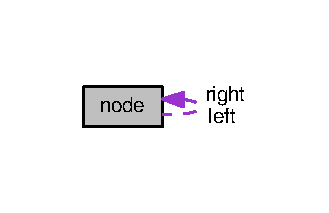
\includegraphics[width=158pt]{structnode__coll__graph}
\end{center}
\end{figure}
\subsection*{Public Attributes}
\begin{DoxyCompactItemize}
\item 
char $\ast$ {\bfseries value}\hypertarget{structnode_a0d2c1eb2a9662a891bb09807232d7f9f}{}\label{structnode_a0d2c1eb2a9662a891bb09807232d7f9f}

\item 
\hyperlink{structnode}{Tree} {\bfseries left}\hypertarget{structnode_a8bb8b7799bf138f227ce9d05ba8d3ca4}{}\label{structnode_a8bb8b7799bf138f227ce9d05ba8d3ca4}

\item 
\hyperlink{structnode}{Tree} {\bfseries right}\hypertarget{structnode_ade8fc5b5eff73152fc0b9c5c6ca6f0dd}{}\label{structnode_ade8fc5b5eff73152fc0b9c5c6ca6f0dd}

\end{DoxyCompactItemize}


The documentation for this struct was generated from the following file\+:\begin{DoxyCompactItemize}
\item 
include/\hyperlink{typedef_8h}{typedef.\+h}\end{DoxyCompactItemize}

\hypertarget{structstackNode}{}\section{stack\+Node Struct Reference}
\label{structstackNode}\index{stack\+Node@{stack\+Node}}


Structure noeud de pile contenant la donnee et le noeud suivant.  




{\ttfamily \#include $<$typedef.\+h$>$}



Collaboration diagram for stack\+Node\+:\nopagebreak
\begin{figure}[H]
\begin{center}
\leavevmode
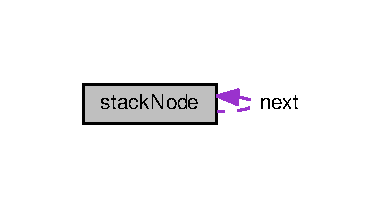
\includegraphics[width=184pt]{structstackNode__coll__graph}
\end{center}
\end{figure}
\subsection*{Public Attributes}
\begin{DoxyCompactItemize}
\item 
char $\ast$ {\bfseries data}\hypertarget{structstackNode_ab8a7f2b607f656ddbdaed84d1c5acbae}{}\label{structstackNode_ab8a7f2b607f656ddbdaed84d1c5acbae}

\item 
\hyperlink{structstackNode}{Stack} {\bfseries next}\hypertarget{structstackNode_a7225663fc2f1d3bad4623de65857c461}{}\label{structstackNode_a7225663fc2f1d3bad4623de65857c461}

\end{DoxyCompactItemize}


\subsection{Detailed Description}
Structure noeud de pile contenant la donnee et le noeud suivant. 

The documentation for this struct was generated from the following file\+:\begin{DoxyCompactItemize}
\item 
include/\hyperlink{typedef_8h}{typedef.\+h}\end{DoxyCompactItemize}

\hypertarget{structstackTree}{}\section{stack\+Tree Struct Reference}
\label{structstackTree}\index{stack\+Tree@{stack\+Tree}}


Collaboration diagram for stack\+Tree\+:\nopagebreak
\begin{figure}[H]
\begin{center}
\leavevmode
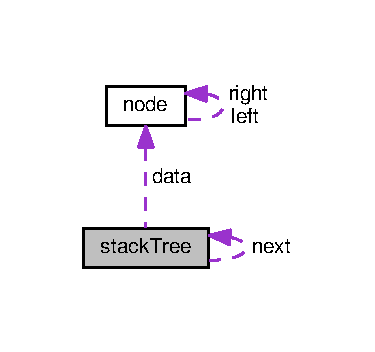
\includegraphics[width=180pt]{structstackTree__coll__graph}
\end{center}
\end{figure}
\subsection*{Public Attributes}
\begin{DoxyCompactItemize}
\item 
\hyperlink{structnode}{Tree} {\bfseries data}\hypertarget{structstackTree_a0948f3bec59d376fcb496088ef1eb390}{}\label{structstackTree_a0948f3bec59d376fcb496088ef1eb390}

\item 
\hyperlink{structstackTree}{Stack\+Tree} {\bfseries next}\hypertarget{structstackTree_ab01d5af00bf143c04cdb6c03ff3b4fb5}{}\label{structstackTree_ab01d5af00bf143c04cdb6c03ff3b4fb5}

\end{DoxyCompactItemize}


The documentation for this struct was generated from the following file\+:\begin{DoxyCompactItemize}
\item 
include/\hyperlink{typedef_8h}{typedef.\+h}\end{DoxyCompactItemize}

\hypertarget{structtree}{}\section{tree Struct Reference}
\label{structtree}\index{tree@{tree}}


Structure d\textquotesingle{}arbre binaire.  




{\ttfamily \#include $<$typedef.\+h$>$}



\subsection{Detailed Description}
Structure d\textquotesingle{}arbre binaire. 

The documentation for this struct was generated from the following file\+:\begin{DoxyCompactItemize}
\item 
include/\hyperlink{typedef_8h}{typedef.\+h}\end{DoxyCompactItemize}

\chapter{File Documentation}
\hypertarget{builtin_8h}{}\section{include/builtin.h File Reference}
\label{builtin_8h}\index{include/builtin.\+h@{include/builtin.\+h}}


Fonctions du Shell.  


{\ttfamily \#include \char`\"{}typedef.\+h\char`\"{}}\\*
Include dependency graph for builtin.\+h\+:\nopagebreak
\begin{figure}[H]
\begin{center}
\leavevmode
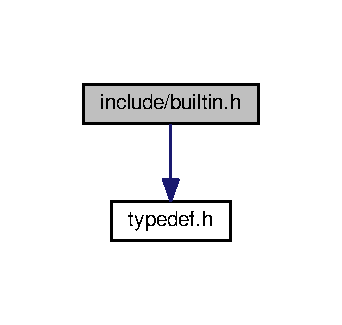
\includegraphics[width=164pt]{builtin_8h__incl}
\end{center}
\end{figure}
\subsection*{Functions}
\begin{DoxyCompactItemize}
\item 
void \hyperlink{builtin_8h_ac2badb93ccbe02d9462229285fc0184b}{cd\+Cmd} (char $\ast$$\ast$arg)
\begin{DoxyCompactList}\small\item\em Reproduit la commande \char`\"{}cd\char`\"{}. \end{DoxyCompactList}\item 
void \hyperlink{builtin_8h_a7363ac1891ce8f70c4c548aaebb16d24}{pwd\+Cmd} ()
\begin{DoxyCompactList}\small\item\em Reproduit la commande \char`\"{}pwd\char`\"{}. \end{DoxyCompactList}\item 
void \hyperlink{builtin_8h_ac9aab741f67d8c4ed42dff107e1cabdd}{exit\+Cmd} ()\hypertarget{builtin_8h_ac9aab741f67d8c4ed42dff107e1cabdd}{}\label{builtin_8h_ac9aab741f67d8c4ed42dff107e1cabdd}

\begin{DoxyCompactList}\small\item\em Quitte le processus courant. \end{DoxyCompactList}\item 
void \hyperlink{builtin_8h_ab2a46d03e0f6275654d6afdb4b092283}{echo\+Cmd} (char $\ast$$\ast$arg)
\begin{DoxyCompactList}\small\item\em Reproduit la commande \char`\"{}echo\char`\"{}. \end{DoxyCompactList}\end{DoxyCompactItemize}


\subsection{Detailed Description}
Fonctions du Shell. 

\begin{DoxyAuthor}{Author}
Loïc.\+B et Jean.\+S
\end{DoxyAuthor}
Reproduction des fonctions du Shell 

\subsection{Function Documentation}
\index{builtin.\+h@{builtin.\+h}!cd\+Cmd@{cd\+Cmd}}
\index{cd\+Cmd@{cd\+Cmd}!builtin.\+h@{builtin.\+h}}
\subsubsection[{\texorpdfstring{cd\+Cmd(char $\ast$$\ast$arg)}{cdCmd(char **arg)}}]{\setlength{\rightskip}{0pt plus 5cm}char $\ast$ cd\+Cmd (
\begin{DoxyParamCaption}
\item[{char $\ast$$\ast$}]{arg}
\end{DoxyParamCaption}
)}\hypertarget{builtin_8h_ac2badb93ccbe02d9462229285fc0184b}{}\label{builtin_8h_ac2badb93ccbe02d9462229285fc0184b}


Reproduit la commande \char`\"{}cd\char`\"{}. 


\begin{DoxyParams}{Parameters}
{\em Chemin} & du répertoire cible \\
\hline
\end{DoxyParams}
\begin{DoxyReturn}{Returns}
Chemin du répertoire cible 
\end{DoxyReturn}
\index{builtin.\+h@{builtin.\+h}!echo\+Cmd@{echo\+Cmd}}
\index{echo\+Cmd@{echo\+Cmd}!builtin.\+h@{builtin.\+h}}
\subsubsection[{\texorpdfstring{echo\+Cmd(char $\ast$$\ast$arg)}{echoCmd(char **arg)}}]{\setlength{\rightskip}{0pt plus 5cm}void echo\+Cmd (
\begin{DoxyParamCaption}
\item[{char $\ast$$\ast$}]{arg}
\end{DoxyParamCaption}
)}\hypertarget{builtin_8h_ab2a46d03e0f6275654d6afdb4b092283}{}\label{builtin_8h_ab2a46d03e0f6275654d6afdb4b092283}


Reproduit la commande \char`\"{}echo\char`\"{}. 


\begin{DoxyParams}{Parameters}
{\em Chaîne} & à afficher \\
\hline
\end{DoxyParams}
\begin{DoxyReturn}{Returns}
Chaîne à afficher 
\end{DoxyReturn}
\index{builtin.\+h@{builtin.\+h}!pwd\+Cmd@{pwd\+Cmd}}
\index{pwd\+Cmd@{pwd\+Cmd}!builtin.\+h@{builtin.\+h}}
\subsubsection[{\texorpdfstring{pwd\+Cmd()}{pwdCmd()}}]{\setlength{\rightskip}{0pt plus 5cm}void pwd\+Cmd (
\begin{DoxyParamCaption}
{}
\end{DoxyParamCaption}
)}\hypertarget{builtin_8h_a7363ac1891ce8f70c4c548aaebb16d24}{}\label{builtin_8h_a7363ac1891ce8f70c4c548aaebb16d24}


Reproduit la commande \char`\"{}pwd\char`\"{}. 

\begin{DoxyReturn}{Returns}
Chemin du répertoire courant 
\end{DoxyReturn}

\hypertarget{parser_8h}{}\section{include/parser.h File Reference}
\label{parser_8h}\index{include/parser.\+h@{include/parser.\+h}}


Gestion du Shell.  


{\ttfamily \#include \char`\"{}typedef.\+h\char`\"{}}\\*
Include dependency graph for parser.\+h\+:
\nopagebreak
\begin{figure}[H]
\begin{center}
\leavevmode
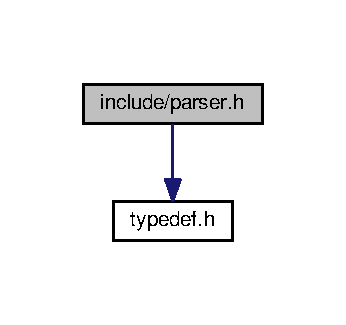
\includegraphics[width=166pt]{parser_8h__incl}
\end{center}
\end{figure}
\subsection*{Functions}
\begin{DoxyCompactItemize}
\item 
int {\bfseries parse\+String\+By\+Sep} (char $\ast$arg, char $\ast$$\ast$parsed, char $\ast$sep)\hypertarget{parser_8h_a456dd62605f1ae7895558a1db7692faf}{}\label{parser_8h_a456dd62605f1ae7895558a1db7692faf}

\item 
int \hyperlink{parser_8h_a7f017fe174474f089db38bc8711a0726}{parse\+String\+By\+Spaces} (char $\ast$arg, char $\ast$$\ast$parsed)
\begin{DoxyCompactList}\small\item\em Découpe la chaîne par la chaîne spécifié \end{DoxyCompactList}\item 
int \hyperlink{parser_8h_ae2fd2e91f032ebee234b6d2e6aae0bdf}{parse\+String\+By\+Special\+Chars} (char $\ast$$\ast$parsed, char $\ast$$\ast$result, int size)
\begin{DoxyCompactList}\small\item\em Découpe la chaîne par caractère special. \end{DoxyCompactList}\item 
void \hyperlink{parser_8h_aba964f39ec7b770c9e6ce65f3214b9ae}{add\+Node\+Stack\+Tree} (\hyperlink{structstackTree}{Stack\+Tree} stack, char $\ast$operator)\hypertarget{parser_8h_aba964f39ec7b770c9e6ce65f3214b9ae}{}\label{parser_8h_aba964f39ec7b770c9e6ce65f3214b9ae}

\begin{DoxyCompactList}\small\item\em Ajoute des noeuds à l\textquotesingle{}arbre. \end{DoxyCompactList}\item 
\hyperlink{structnode}{Tree} \hyperlink{parser_8h_aeef948f3c1413d818faf4cddad49c46c}{parse\+String\+To\+Stacks} (char $\ast$$\ast$parsed, int size\+Parsed)\hypertarget{parser_8h_aeef948f3c1413d818faf4cddad49c46c}{}\label{parser_8h_aeef948f3c1413d818faf4cddad49c46c}

\begin{DoxyCompactList}\small\item\em Construit l\textquotesingle{}arbre syntaxique. \end{DoxyCompactList}\item 
void {\bfseries remove\+All\+Chars} (char $\ast$str, char c)\hypertarget{parser_8h_a20e3dd4792062941cced7d59e1578593}{}\label{parser_8h_a20e3dd4792062941cced7d59e1578593}

\end{DoxyCompactItemize}


\subsection{Detailed Description}
Gestion du Shell. 

\begin{DoxyAuthor}{Author}
Loïc.\+B et Jean.\+S
\end{DoxyAuthor}
Gestion du Shell et de l\textquotesingle{}I\+HM 

\subsection{Function Documentation}
\index{parser.\+h@{parser.\+h}!parse\+String\+By\+Spaces@{parse\+String\+By\+Spaces}}
\index{parse\+String\+By\+Spaces@{parse\+String\+By\+Spaces}!parser.\+h@{parser.\+h}}
\subsubsection[{\texorpdfstring{parse\+String\+By\+Spaces(char $\ast$arg, char $\ast$$\ast$parsed)}{parseStringBySpaces(char *arg, char **parsed)}}]{\setlength{\rightskip}{0pt plus 5cm}void parse\+String\+By\+Spaces (
\begin{DoxyParamCaption}
\item[{char $\ast$}]{arg, }
\item[{char $\ast$$\ast$}]{parsed}
\end{DoxyParamCaption}
)}\hypertarget{parser_8h_a7f017fe174474f089db38bc8711a0726}{}\label{parser_8h_a7f017fe174474f089db38bc8711a0726}


Découpe la chaîne par la chaîne spécifié 

Découpe la chaîne par caractère espace.

\begin{DoxyReturn}{Returns}
argc 
\end{DoxyReturn}
\index{parser.\+h@{parser.\+h}!parse\+String\+By\+Special\+Chars@{parse\+String\+By\+Special\+Chars}}
\index{parse\+String\+By\+Special\+Chars@{parse\+String\+By\+Special\+Chars}!parser.\+h@{parser.\+h}}
\subsubsection[{\texorpdfstring{parse\+String\+By\+Special\+Chars(char $\ast$$\ast$parsed, char $\ast$$\ast$result, int size)}{parseStringBySpecialChars(char **parsed, char **result, int size)}}]{\setlength{\rightskip}{0pt plus 5cm}int parse\+String\+By\+Special\+Chars (
\begin{DoxyParamCaption}
\item[{char $\ast$$\ast$}]{parsed, }
\item[{char $\ast$$\ast$}]{result, }
\item[{int}]{size}
\end{DoxyParamCaption}
)}\hypertarget{parser_8h_ae2fd2e91f032ebee234b6d2e6aae0bdf}{}\label{parser_8h_ae2fd2e91f032ebee234b6d2e6aae0bdf}


Découpe la chaîne par caractère special. 

\begin{DoxyReturn}{Returns}
argc 
\end{DoxyReturn}

\hypertarget{shell_8h}{}\section{include/shell.h File Reference}
\label{shell_8h}\index{include/shell.\+h@{include/shell.\+h}}


Gestion du Shell.  


{\ttfamily \#include \char`\"{}typedef.\+h\char`\"{}}\\*
Include dependency graph for shell.\+h\+:
\nopagebreak
\begin{figure}[H]
\begin{center}
\leavevmode
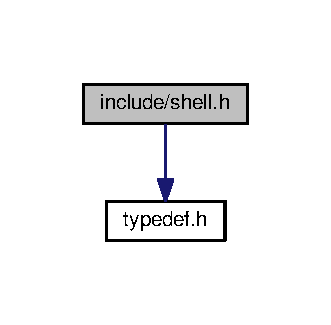
\includegraphics[width=159pt]{shell_8h__incl}
\end{center}
\end{figure}
\subsection*{Macros}
\begin{DoxyCompactItemize}
\item 
\#define {\bfseries \+\_\+\+S\+H\+E\+L\+L\+\_\+\+H\+\_\+}~/$\ast$ Edit suite aux corrections des posts suivants -\/$>$ $\ast$/\hypertarget{shell_8h_af6d1298673e2abca2dc62735d4b8b949}{}\label{shell_8h_af6d1298673e2abca2dc62735d4b8b949}

\end{DoxyCompactItemize}
\subsection*{Functions}
\begin{DoxyCompactItemize}
\item 
void \hyperlink{shell_8h_aba0e7cbf36b01d94dd5d0b8a5e3e1c2b}{shell\+Reader} ()\hypertarget{shell_8h_aba0e7cbf36b01d94dd5d0b8a5e3e1c2b}{}\label{shell_8h_aba0e7cbf36b01d94dd5d0b8a5e3e1c2b}

\begin{DoxyCompactList}\small\item\em Fonction de lecture des commande en boucle sur la console. \end{DoxyCompactList}\item 
void {\bfseries read\+Input} (char $\ast$command, int size)\hypertarget{shell_8h_af8493e88dd434853720a81098bf83a3a}{}\label{shell_8h_af8493e88dd434853720a81098bf83a3a}

\item 
int \hyperlink{shell_8h_a11b419f784bac628d7bbe2c8c2c5e21a}{readerL} (char $\ast$chaine, int longueur)
\begin{DoxyCompactList}\small\item\em Lecture des elements renseignes par l\textquotesingle{}utilisateur afin d\textquotesingle{}executer les commandes avec ses parametres. \end{DoxyCompactList}\item 
int \hyperlink{shell_8h_ae6a056a6f5706bd9d625cb813f9e8c8f}{end\+Of\+Command} (char $\ast$chaine, int longueur)
\begin{DoxyCompactList}\small\item\em Permet de savoir si la chaine contient le caractere de fin de chaine. \end{DoxyCompactList}\item 
void \hyperlink{shell_8h_a750be53afe22b006b8b36b42f3c12323}{clean\+Buffer} ()\hypertarget{shell_8h_a750be53afe22b006b8b36b42f3c12323}{}\label{shell_8h_a750be53afe22b006b8b36b42f3c12323}

\begin{DoxyCompactList}\small\item\em Vide le buffer. \end{DoxyCompactList}\item 
\hyperlink{typedef_8h_af6a258d8f3ee5206d682d799316314b1}{bool} {\bfseries call\+Commands} (char $\ast$$\ast$argv)\hypertarget{shell_8h_abc4c8860ec6ba2bcfaa0fdebad5e896b}{}\label{shell_8h_abc4c8860ec6ba2bcfaa0fdebad5e896b}

\item 
\hyperlink{typedef_8h_af6a258d8f3ee5206d682d799316314b1}{bool} \hyperlink{shell_8h_ac95dace850d5e2589b1b3ac07bd8ec1b}{execute\+Command} (char $\ast$$\ast$argv)
\begin{DoxyCompactList}\small\item\em Délègue l\textquotesingle{}appel via fork/execvp à un processus fils. \end{DoxyCompactList}\item 
\hyperlink{typedef_8h_af6a258d8f3ee5206d682d799316314b1}{bool} {\bfseries execute} (char $\ast$$\ast$argv)\hypertarget{shell_8h_ab7b0baacd76c74612196051b9c12ed74}{}\label{shell_8h_ab7b0baacd76c74612196051b9c12ed74}

\item 
void {\bfseries historize} (char $\ast$arg)\hypertarget{shell_8h_a85d9d45d2aa5de73f0eec26eb8543803}{}\label{shell_8h_a85d9d45d2aa5de73f0eec26eb8543803}

\item 
void {\bfseries print\+Working\+Dir\+Colored} ()\hypertarget{shell_8h_aab4dd3d9c3ee9edc0913c58b6d3d63f3}{}\label{shell_8h_aab4dd3d9c3ee9edc0913c58b6d3d63f3}

\item 
void {\bfseries decrypt\+Args} (char $\ast$cmd, char $\ast$$\ast$params)\hypertarget{shell_8h_a81e3530b03d4772faf566484db0ee62a}{}\label{shell_8h_a81e3530b03d4772faf566484db0ee62a}

\item 
\hyperlink{typedef_8h_af6a258d8f3ee5206d682d799316314b1}{bool} \hyperlink{shell_8h_ae2b795612ce582293c9c2e58492d161e}{evaluate\+Tree} (\hyperlink{structnode}{Tree} t)
\begin{DoxyCompactList}\small\item\em Permet d\textquotesingle{}evaluer l\textquotesingle{}arbre compose des commandes et operateurs. \end{DoxyCompactList}\item 
void {\bfseries process\+Commands} (char $\ast$$\ast$argv, int argc)\hypertarget{shell_8h_ac92c8e7f98071905150a302360d0717c}{}\label{shell_8h_ac92c8e7f98071905150a302360d0717c}

\end{DoxyCompactItemize}


\subsection{Detailed Description}
Gestion du Shell. 

\begin{DoxyAuthor}{Author}
Loïc.\+B et Jean.\+S
\end{DoxyAuthor}
Gestion du Shell et de l\textquotesingle{}I\+HM 

\subsection{Function Documentation}
\index{shell.\+h@{shell.\+h}!end\+Of\+Command@{end\+Of\+Command}}
\index{end\+Of\+Command@{end\+Of\+Command}!shell.\+h@{shell.\+h}}
\subsubsection[{\texorpdfstring{end\+Of\+Command(char $\ast$chaine, int longueur)}{endOfCommand(char *chaine, int longueur)}}]{\setlength{\rightskip}{0pt plus 5cm}int end\+Of\+Command (
\begin{DoxyParamCaption}
\item[{char $\ast$}]{chaine, }
\item[{int}]{longueur}
\end{DoxyParamCaption}
)}\hypertarget{shell_8h_ae6a056a6f5706bd9d625cb813f9e8c8f}{}\label{shell_8h_ae6a056a6f5706bd9d625cb813f9e8c8f}


Permet de savoir si la chaine contient le caractere de fin de chaine. 


\begin{DoxyParams}{Parameters}
{\em Chaîne} & d\textquotesingle{}entrée \\
\hline
{\em Longueur} & de la chaîne d\textquotesingle{}entrée \\
\hline
\end{DoxyParams}
\begin{DoxyReturn}{Returns}
int 1 si caract de fin, 0 sinon 
\end{DoxyReturn}
\index{shell.\+h@{shell.\+h}!evaluate\+Tree@{evaluate\+Tree}}
\index{evaluate\+Tree@{evaluate\+Tree}!shell.\+h@{shell.\+h}}
\subsubsection[{\texorpdfstring{evaluate\+Tree(\+Tree t)}{evaluateTree(Tree t)}}]{\setlength{\rightskip}{0pt plus 5cm}char $\ast$ evaluate\+Tree (
\begin{DoxyParamCaption}
\item[{{\bf Tree}}]{t}
\end{DoxyParamCaption}
)}\hypertarget{shell_8h_ae2b795612ce582293c9c2e58492d161e}{}\label{shell_8h_ae2b795612ce582293c9c2e58492d161e}


Permet d\textquotesingle{}evaluer l\textquotesingle{}arbre compose des commandes et operateurs. 

Permet d\textquotesingle{}executer la commande et d\textquotesingle{}evaluer si cette derniere doit s\textquotesingle{}executer en arriere plan.


\begin{DoxyParams}{Parameters}
{\em Tree} & noeud a évaluer \\
\hline
\end{DoxyParams}
\begin{DoxyReturn}{Returns}
resultat d\textquotesingle{}exécution du noeuf passé en paramètre 
\end{DoxyReturn}
\index{shell.\+h@{shell.\+h}!execute\+Command@{execute\+Command}}
\index{execute\+Command@{execute\+Command}!shell.\+h@{shell.\+h}}
\subsubsection[{\texorpdfstring{execute\+Command(char $\ast$$\ast$argv)}{executeCommand(char **argv)}}]{\setlength{\rightskip}{0pt plus 5cm}{\bf bool} execute\+Command (
\begin{DoxyParamCaption}
\item[{char $\ast$$\ast$}]{argv}
\end{DoxyParamCaption}
)}\hypertarget{shell_8h_ac95dace850d5e2589b1b3ac07bd8ec1b}{}\label{shell_8h_ac95dace850d5e2589b1b3ac07bd8ec1b}


Délègue l\textquotesingle{}appel via fork/execvp à un processus fils. 

Redirige l\textquotesingle{}execution des cmds vers les commandes programmees maison quand c\textquotesingle{}est necessaire.


\begin{DoxyParams}{Parameters}
{\em Chaîne} & d\textquotesingle{}entrée\\
\hline
{\em Chaîne} & d\textquotesingle{}entrée, cmd + args \\
\hline
\end{DoxyParams}
\index{shell.\+h@{shell.\+h}!readerL@{readerL}}
\index{readerL@{readerL}!shell.\+h@{shell.\+h}}
\subsubsection[{\texorpdfstring{reader\+L(char $\ast$chaine, int longueur)}{readerL(char *chaine, int longueur)}}]{\setlength{\rightskip}{0pt plus 5cm}int readerL (
\begin{DoxyParamCaption}
\item[{char $\ast$}]{chaine, }
\item[{int}]{longueur}
\end{DoxyParamCaption}
)}\hypertarget{shell_8h_a11b419f784bac628d7bbe2c8c2c5e21a}{}\label{shell_8h_a11b419f784bac628d7bbe2c8c2c5e21a}


Lecture des elements renseignes par l\textquotesingle{}utilisateur afin d\textquotesingle{}executer les commandes avec ses parametres. 


\begin{DoxyParams}{Parameters}
{\em Chaîne} & d\textquotesingle{}entrée \\
\hline
{\em Longueur} & de la chaîne d\textquotesingle{}entrée \\
\hline
\end{DoxyParams}
\begin{DoxyReturn}{Returns}
resultat 
\end{DoxyReturn}

\hypertarget{stack_8h}{}\section{include/stack.h File Reference}
\label{stack_8h}\index{include/stack.\+h@{include/stack.\+h}}


Pile contenant des strings (et on parle bien des chaînes de caractères ;))  


{\ttfamily \#include \char`\"{}../include/typedef.\+h\char`\"{}}\\*
Include dependency graph for stack.\+h\+:\nopagebreak
\begin{figure}[H]
\begin{center}
\leavevmode
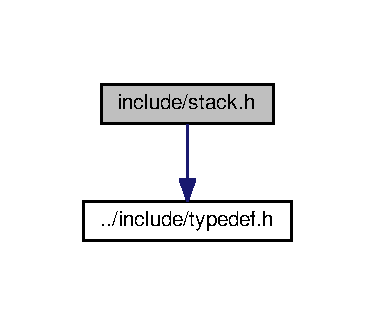
\includegraphics[width=180pt]{stack_8h__incl}
\end{center}
\end{figure}
\subsection*{Functions}
\begin{DoxyCompactItemize}
\item 
\hyperlink{structstackNode}{Stack} \hyperlink{stack_8h_ada4fdce0f2ef228b35f9eb95c11f9c9a}{new\+Node} (char $\ast$data)
\begin{DoxyCompactList}\small\item\em Initialise une pile. \end{DoxyCompactList}\item 
\hyperlink{typedef_8h_af6a258d8f3ee5206d682d799316314b1}{bool} \hyperlink{stack_8h_ac102d81076e3ce7701a82e5a91486a1d}{empty} (\hyperlink{structstackNode}{Stack} \hyperlink{tree_8h_a66fb9b676a07f944e35a2171cff66e4b}{root})
\begin{DoxyCompactList}\small\item\em Si pile vide renvoi 0. \end{DoxyCompactList}\item 
void \hyperlink{stack_8h_a85ae875d8d9cd3bbf0b3460de1c03df2}{push} (\hyperlink{structstackNode}{Stack} $\ast$\hyperlink{tree_8h_a66fb9b676a07f944e35a2171cff66e4b}{root}, char $\ast$data)
\begin{DoxyCompactList}\small\item\em Ajoute un élément à la pile passée en paramètre. \end{DoxyCompactList}\item 
char $\ast$ \hyperlink{stack_8h_a027d41b75da5f59c4e0fc39c50e9c6c5}{pop} (\hyperlink{structstackNode}{Stack} $\ast$\hyperlink{tree_8h_a66fb9b676a07f944e35a2171cff66e4b}{root})
\begin{DoxyCompactList}\small\item\em Enlève l\textquotesingle{}élement au sommet de la pile et renvoi son contenu. \end{DoxyCompactList}\end{DoxyCompactItemize}


\subsection{Detailed Description}
Pile contenant des strings (et on parle bien des chaînes de caractères ;)) 

\begin{DoxyAuthor}{Author}
Loïc B. 
\end{DoxyAuthor}


\subsection{Function Documentation}
\index{stack.\+h@{stack.\+h}!empty@{empty}}
\index{empty@{empty}!stack.\+h@{stack.\+h}}
\subsubsection[{\texorpdfstring{empty(\+Stack root)}{empty(Stack root)}}]{\setlength{\rightskip}{0pt plus 5cm}{\bf bool} empty (
\begin{DoxyParamCaption}
\item[{{\bf Stack}}]{root}
\end{DoxyParamCaption}
)}\hypertarget{stack_8h_ac102d81076e3ce7701a82e5a91486a1d}{}\label{stack_8h_ac102d81076e3ce7701a82e5a91486a1d}


Si pile vide renvoi 0. 


\begin{DoxyParams}{Parameters}
{\em Stack} & \\
\hline
\end{DoxyParams}
\begin{DoxyReturn}{Returns}
bool 
\end{DoxyReturn}
\index{stack.\+h@{stack.\+h}!new\+Node@{new\+Node}}
\index{new\+Node@{new\+Node}!stack.\+h@{stack.\+h}}
\subsubsection[{\texorpdfstring{new\+Node(char $\ast$data)}{newNode(char *data)}}]{\setlength{\rightskip}{0pt plus 5cm}{\bf Stack} new\+Node (
\begin{DoxyParamCaption}
\item[{char $\ast$}]{data}
\end{DoxyParamCaption}
)}\hypertarget{stack_8h_ada4fdce0f2ef228b35f9eb95c11f9c9a}{}\label{stack_8h_ada4fdce0f2ef228b35f9eb95c11f9c9a}


Initialise une pile. 


\begin{DoxyParams}{Parameters}
{\em char$\ast$} & donnée à stocker \\
\hline
\end{DoxyParams}
\begin{DoxyReturn}{Returns}
Stack 
\end{DoxyReturn}
\index{stack.\+h@{stack.\+h}!pop@{pop}}
\index{pop@{pop}!stack.\+h@{stack.\+h}}
\subsubsection[{\texorpdfstring{pop(\+Stack $\ast$root)}{pop(Stack *root)}}]{\setlength{\rightskip}{0pt plus 5cm}char $\ast$ pop (
\begin{DoxyParamCaption}
\item[{{\bf Stack} $\ast$}]{root}
\end{DoxyParamCaption}
)}\hypertarget{stack_8h_a027d41b75da5f59c4e0fc39c50e9c6c5}{}\label{stack_8h_a027d41b75da5f59c4e0fc39c50e9c6c5}


Enlève l\textquotesingle{}élement au sommet de la pile et renvoi son contenu. 


\begin{DoxyParams}{Parameters}
{\em Stack} & \\
\hline
\end{DoxyParams}
\begin{DoxyReturn}{Returns}
char$\ast$ data 
\end{DoxyReturn}
\index{stack.\+h@{stack.\+h}!push@{push}}
\index{push@{push}!stack.\+h@{stack.\+h}}
\subsubsection[{\texorpdfstring{push(\+Stack $\ast$root, char $\ast$data)}{push(Stack *root, char *data)}}]{\setlength{\rightskip}{0pt plus 5cm}void push (
\begin{DoxyParamCaption}
\item[{{\bf Stack} $\ast$}]{root, }
\item[{char $\ast$}]{data}
\end{DoxyParamCaption}
)}\hypertarget{stack_8h_a85ae875d8d9cd3bbf0b3460de1c03df2}{}\label{stack_8h_a85ae875d8d9cd3bbf0b3460de1c03df2}


Ajoute un élément à la pile passée en paramètre. 


\begin{DoxyParams}{Parameters}
{\em Stack$\ast$} & la pile et char$\ast$ la donnée \\
\hline
\end{DoxyParams}

\hypertarget{stackTree_8h}{}\section{include/stack\+Tree.h File Reference}
\label{stackTree_8h}\index{include/stack\+Tree.\+h@{include/stack\+Tree.\+h}}


Pile contenant des arbres.  


{\ttfamily \#include \char`\"{}../include/typedef.\+h\char`\"{}}\\*
Include dependency graph for stack\+Tree.\+h\+:\nopagebreak
\begin{figure}[H]
\begin{center}
\leavevmode
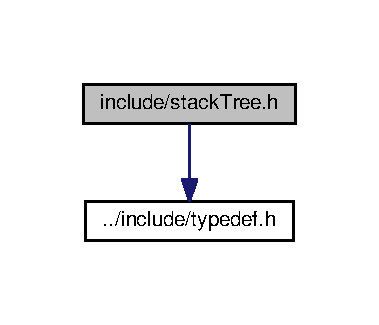
\includegraphics[width=182pt]{stackTree_8h__incl}
\end{center}
\end{figure}
\subsection*{Functions}
\begin{DoxyCompactItemize}
\item 
\hyperlink{structstackTree}{Stack\+Tree} \hyperlink{stackTree_8h_ac7860315aeb4e2ba097574b9e293146f}{new\+Node\+Stack\+Tree} (\hyperlink{structnode}{Tree} data)
\begin{DoxyCompactList}\small\item\em Initialise une pile. \end{DoxyCompactList}\item 
\hyperlink{typedef_8h_af6a258d8f3ee5206d682d799316314b1}{bool} \hyperlink{stackTree_8h_a3e101266a4325d242ea73417931989f5}{is\+Empty\+Stack\+Tree} (\hyperlink{structstackTree}{Stack\+Tree} \hyperlink{tree_8h_a66fb9b676a07f944e35a2171cff66e4b}{root})
\begin{DoxyCompactList}\small\item\em Si pile vide renvoi 0. \end{DoxyCompactList}\item 
void \hyperlink{stackTree_8h_a8be59de159b13bbbac7ccaf531c3f638}{push\+Stack\+Tree} (\hyperlink{structstackTree}{Stack\+Tree} $\ast$\hyperlink{tree_8h_a66fb9b676a07f944e35a2171cff66e4b}{root}, \hyperlink{structnode}{Tree} data)
\begin{DoxyCompactList}\small\item\em Ajoute un élément à la pile passée en paramètre. \end{DoxyCompactList}\item 
\hyperlink{structnode}{Tree} \hyperlink{stackTree_8h_a072fcedcbe8214ca0dc0918e2ab3c309}{pop\+Stack\+Tree} (\hyperlink{structstackTree}{Stack\+Tree} $\ast$\hyperlink{tree_8h_a66fb9b676a07f944e35a2171cff66e4b}{root})
\begin{DoxyCompactList}\small\item\em Enlève l\textquotesingle{}élement au sommet de la pile et renvoi son contenu. \end{DoxyCompactList}\item 
\hyperlink{structnode}{Tree} \hyperlink{stackTree_8h_a857f386c967b559a2b55013bda48ec00}{peek\+Stack\+Tree} (\hyperlink{structstackTree}{Stack\+Tree} \hyperlink{tree_8h_a66fb9b676a07f944e35a2171cff66e4b}{root})
\begin{DoxyCompactList}\small\item\em Renvoi la donnée de l\textquotesingle{}élement au sommet de la pile. \end{DoxyCompactList}\end{DoxyCompactItemize}


\subsection{Detailed Description}
Pile contenant des arbres. 

\begin{DoxyAuthor}{Author}
Loïc.\+B et Jean.\+S 
\end{DoxyAuthor}


\subsection{Function Documentation}
\index{stack\+Tree.\+h@{stack\+Tree.\+h}!is\+Empty\+Stack\+Tree@{is\+Empty\+Stack\+Tree}}
\index{is\+Empty\+Stack\+Tree@{is\+Empty\+Stack\+Tree}!stack\+Tree.\+h@{stack\+Tree.\+h}}
\subsubsection[{\texorpdfstring{is\+Empty\+Stack\+Tree(\+Stack\+Tree root)}{isEmptyStackTree(StackTree root)}}]{\setlength{\rightskip}{0pt plus 5cm}{\bf bool} is\+Empty\+Stack\+Tree (
\begin{DoxyParamCaption}
\item[{{\bf Stack\+Tree}}]{root}
\end{DoxyParamCaption}
)}\hypertarget{stackTree_8h_a3e101266a4325d242ea73417931989f5}{}\label{stackTree_8h_a3e101266a4325d242ea73417931989f5}


Si pile vide renvoi 0. 


\begin{DoxyParams}{Parameters}
{\em Stack\+Tree} & \\
\hline
\end{DoxyParams}
\begin{DoxyReturn}{Returns}
bool 
\end{DoxyReturn}
\index{stack\+Tree.\+h@{stack\+Tree.\+h}!new\+Node\+Stack\+Tree@{new\+Node\+Stack\+Tree}}
\index{new\+Node\+Stack\+Tree@{new\+Node\+Stack\+Tree}!stack\+Tree.\+h@{stack\+Tree.\+h}}
\subsubsection[{\texorpdfstring{new\+Node\+Stack\+Tree(\+Tree data)}{newNodeStackTree(Tree data)}}]{\setlength{\rightskip}{0pt plus 5cm}{\bf Stack\+Tree} new\+Node\+Stack\+Tree (
\begin{DoxyParamCaption}
\item[{{\bf Tree}}]{data}
\end{DoxyParamCaption}
)}\hypertarget{stackTree_8h_ac7860315aeb4e2ba097574b9e293146f}{}\label{stackTree_8h_ac7860315aeb4e2ba097574b9e293146f}


Initialise une pile. 


\begin{DoxyParams}{Parameters}
{\em Tree$\ast$} & donnée à stocker \\
\hline
\end{DoxyParams}
\begin{DoxyReturn}{Returns}
Stack\+Tree 
\end{DoxyReturn}
\index{stack\+Tree.\+h@{stack\+Tree.\+h}!peek\+Stack\+Tree@{peek\+Stack\+Tree}}
\index{peek\+Stack\+Tree@{peek\+Stack\+Tree}!stack\+Tree.\+h@{stack\+Tree.\+h}}
\subsubsection[{\texorpdfstring{peek\+Stack\+Tree(\+Stack\+Tree root)}{peekStackTree(StackTree root)}}]{\setlength{\rightskip}{0pt plus 5cm}{\bf Tree} peek\+Stack\+Tree (
\begin{DoxyParamCaption}
\item[{{\bf Stack\+Tree}}]{root}
\end{DoxyParamCaption}
)}\hypertarget{stackTree_8h_a857f386c967b559a2b55013bda48ec00}{}\label{stackTree_8h_a857f386c967b559a2b55013bda48ec00}


Renvoi la donnée de l\textquotesingle{}élement au sommet de la pile. 


\begin{DoxyParams}{Parameters}
{\em Stack\+Tree} & \\
\hline
\end{DoxyParams}
\begin{DoxyReturn}{Returns}
Tree data 
\end{DoxyReturn}
\index{stack\+Tree.\+h@{stack\+Tree.\+h}!pop\+Stack\+Tree@{pop\+Stack\+Tree}}
\index{pop\+Stack\+Tree@{pop\+Stack\+Tree}!stack\+Tree.\+h@{stack\+Tree.\+h}}
\subsubsection[{\texorpdfstring{pop\+Stack\+Tree(\+Stack\+Tree $\ast$root)}{popStackTree(StackTree *root)}}]{\setlength{\rightskip}{0pt plus 5cm}{\bf Tree} pop\+Stack\+Tree (
\begin{DoxyParamCaption}
\item[{{\bf Stack\+Tree} $\ast$}]{root}
\end{DoxyParamCaption}
)}\hypertarget{stackTree_8h_a072fcedcbe8214ca0dc0918e2ab3c309}{}\label{stackTree_8h_a072fcedcbe8214ca0dc0918e2ab3c309}


Enlève l\textquotesingle{}élement au sommet de la pile et renvoi son contenu. 


\begin{DoxyParams}{Parameters}
{\em Stack\+Tree$\ast$} & \\
\hline
\end{DoxyParams}
\begin{DoxyReturn}{Returns}
Tree data 
\end{DoxyReturn}
\index{stack\+Tree.\+h@{stack\+Tree.\+h}!push\+Stack\+Tree@{push\+Stack\+Tree}}
\index{push\+Stack\+Tree@{push\+Stack\+Tree}!stack\+Tree.\+h@{stack\+Tree.\+h}}
\subsubsection[{\texorpdfstring{push\+Stack\+Tree(\+Stack\+Tree $\ast$root, Tree data)}{pushStackTree(StackTree *root, Tree data)}}]{\setlength{\rightskip}{0pt plus 5cm}push\+Stack\+Tree (
\begin{DoxyParamCaption}
\item[{{\bf Stack\+Tree} $\ast$}]{root, }
\item[{{\bf Tree}}]{data}
\end{DoxyParamCaption}
)}\hypertarget{stackTree_8h_a8be59de159b13bbbac7ccaf531c3f638}{}\label{stackTree_8h_a8be59de159b13bbbac7ccaf531c3f638}


Ajoute un élément à la pile passée en paramètre. 


\begin{DoxyParams}{Parameters}
{\em Stack\+Tree$\ast$} & la pile et Tree la donnée \\
\hline
\end{DoxyParams}

\hypertarget{tree_8h}{}\section{include/tree.h File Reference}
\label{tree_8h}\index{include/tree.\+h@{include/tree.\+h}}


Gestion du Shell.  


{\ttfamily \#include \char`\"{}typedef.\+h\char`\"{}}\\*
Include dependency graph for tree.\+h\+:
\nopagebreak
\begin{figure}[H]
\begin{center}
\leavevmode
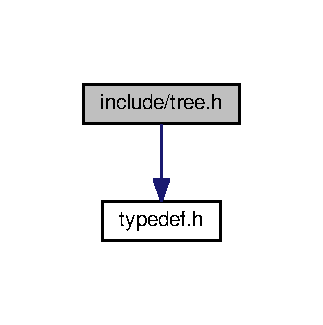
\includegraphics[width=155pt]{tree_8h__incl}
\end{center}
\end{figure}
\subsection*{Macros}
\begin{DoxyCompactItemize}
\item 
\#define {\bfseries \+\_\+\+T\+R\+E\+E\+\_\+\+H\+\_\+}~/$\ast$ Edit suite aux corrections des posts suivants -\/$>$ $\ast$/\hypertarget{tree_8h_ae79288a9c2d6e61b357d8fbc6f6d9e5d}{}\label{tree_8h_ae79288a9c2d6e61b357d8fbc6f6d9e5d}

\end{DoxyCompactItemize}
\subsection*{Functions}
\begin{DoxyCompactItemize}
\item 
\hyperlink{structnode}{Tree} \hyperlink{tree_8h_a39fee9e551235f35ffb7c7c84831cfcf}{create\+Tree} (char $\ast$val, \hyperlink{structnode}{Tree} ls, \hyperlink{structnode}{Tree} rs)
\begin{DoxyCompactList}\small\item\em Cree un arbre. \end{DoxyCompactList}\item 
void \hyperlink{tree_8h_a42de0a8d12e01a75f477b3a6bfac4027}{add\+Node} (\hyperlink{structnode}{Tree} t, char $\ast$val)
\begin{DoxyCompactList}\small\item\em Ajout d\textquotesingle{}un noeud a un arbre. \end{DoxyCompactList}\item 
char $\ast$ \hyperlink{tree_8h_a66fb9b676a07f944e35a2171cff66e4b}{root} (\hyperlink{structnode}{Tree} t)
\begin{DoxyCompactList}\small\item\em Retourne la valeur de l\textquotesingle{}arbre. \end{DoxyCompactList}\item 
void {\bfseries write\+Tree} (\hyperlink{structnode}{Tree} t, F\+I\+LE $\ast$fp)\hypertarget{tree_8h_aa189767efdb91832c3e3005ed5a75e6f}{}\label{tree_8h_aa189767efdb91832c3e3005ed5a75e6f}

\item 
void \hyperlink{tree_8h_a0bd2f6637ff829975a5c0349fc7ee22a}{save\+\_\+dot} (\hyperlink{structnode}{Tree} t, char $\ast$filename)
\begin{DoxyCompactList}\small\item\em dessine la representation de l\textquotesingle{}arbre. \end{DoxyCompactList}\item 
void \hyperlink{tree_8h_ae2f270c14406b7dfaf6b566d643f233a}{display} (\hyperlink{structnode}{Tree} t)\hypertarget{tree_8h_ae2f270c14406b7dfaf6b566d643f233a}{}\label{tree_8h_ae2f270c14406b7dfaf6b566d643f233a}

\begin{DoxyCompactList}\small\item\em affiche la representation de l\textquotesingle{}arbre. \end{DoxyCompactList}\item 
int \hyperlink{tree_8h_ab471c13de30182fb7b9a0e0f2a0b7d6e}{size\+Tree} (\hyperlink{structnode}{Tree} t)
\begin{DoxyCompactList}\small\item\em Calcul la taille de l\textquotesingle{}arbre. \end{DoxyCompactList}\item 
\hyperlink{typedef_8h_af6a258d8f3ee5206d682d799316314b1}{bool} \hyperlink{tree_8h_ae4ea4d4d609b15ac54146adeb64eb435}{is\+Empty} (\hyperlink{structnode}{Tree} t)
\begin{DoxyCompactList}\small\item\em Test si l\textquotesingle{}arbre est vide. \end{DoxyCompactList}\item 
\hyperlink{structnode}{Tree} {\bfseries left} (\hyperlink{structnode}{Tree} t)\hypertarget{tree_8h_a626356b3c8f3e0130d0e043a1dd8547c}{}\label{tree_8h_a626356b3c8f3e0130d0e043a1dd8547c}

\item 
\hyperlink{structnode}{Tree} {\bfseries right} (\hyperlink{structnode}{Tree} t)\hypertarget{tree_8h_a098460d0916242eebda50610e2a86e39}{}\label{tree_8h_a098460d0916242eebda50610e2a86e39}

\item 
\hyperlink{typedef_8h_af6a258d8f3ee5206d682d799316314b1}{bool} {\bfseries is\+Leaf} (\hyperlink{structnode}{Tree} t)\hypertarget{tree_8h_ae932bf12c2804f0f647c68a32038191c}{}\label{tree_8h_ae932bf12c2804f0f647c68a32038191c}

\item 
void \hyperlink{tree_8h_a47969070eb9b124b455b59d587f66bb4}{parcours\+Prefixe} (\hyperlink{structnode}{Tree} a)
\begin{DoxyCompactList}\small\item\em Parcours l\textquotesingle{}arbre e manière préfixé et affiche l\textquotesingle{}arbre. \end{DoxyCompactList}\end{DoxyCompactItemize}


\subsection{Detailed Description}
Gestion du Shell. 

\begin{DoxyAuthor}{Author}
Loïc.\+B et Jean.\+S
\end{DoxyAuthor}
Gestion du Shell et de l\textquotesingle{}I\+HM 

\subsection{Function Documentation}
\index{tree.\+h@{tree.\+h}!add\+Node@{add\+Node}}
\index{add\+Node@{add\+Node}!tree.\+h@{tree.\+h}}
\subsubsection[{\texorpdfstring{add\+Node(\+Tree t, char $\ast$val)}{addNode(Tree t, char *val)}}]{\setlength{\rightskip}{0pt plus 5cm}void add\+Node (
\begin{DoxyParamCaption}
\item[{{\bf Tree}}]{t, }
\item[{char $\ast$}]{val}
\end{DoxyParamCaption}
)}\hypertarget{tree_8h_a42de0a8d12e01a75f477b3a6bfac4027}{}\label{tree_8h_a42de0a8d12e01a75f477b3a6bfac4027}


Ajout d\textquotesingle{}un noeud a un arbre. 


\begin{DoxyParams}{Parameters}
{\em Tree} & t arbre source, char$\ast$ val valeur du noeud \\
\hline
\end{DoxyParams}
\index{tree.\+h@{tree.\+h}!create\+Tree@{create\+Tree}}
\index{create\+Tree@{create\+Tree}!tree.\+h@{tree.\+h}}
\subsubsection[{\texorpdfstring{create\+Tree(char $\ast$val, Tree ls, Tree rs)}{createTree(char *val, Tree ls, Tree rs)}}]{\setlength{\rightskip}{0pt plus 5cm}{\bf Tree} create\+Tree (
\begin{DoxyParamCaption}
\item[{char $\ast$}]{val, }
\item[{{\bf Tree}}]{ls, }
\item[{{\bf Tree}}]{rs}
\end{DoxyParamCaption}
)}\hypertarget{tree_8h_a39fee9e551235f35ffb7c7c84831cfcf}{}\label{tree_8h_a39fee9e551235f35ffb7c7c84831cfcf}


Cree un arbre. 


\begin{DoxyParams}{Parameters}
{\em char$\ast$} & valeur du noeud, Tree ls arbre de gauche,Tree ls arbre de droite \\
\hline
\end{DoxyParams}
\begin{DoxyReturn}{Returns}
Tree \+: retourne l\textquotesingle{}arbre cree 
\end{DoxyReturn}
\index{tree.\+h@{tree.\+h}!is\+Empty@{is\+Empty}}
\index{is\+Empty@{is\+Empty}!tree.\+h@{tree.\+h}}
\subsubsection[{\texorpdfstring{is\+Empty(\+Tree t)}{isEmpty(Tree t)}}]{\setlength{\rightskip}{0pt plus 5cm}{\bf bool} is\+Empty (
\begin{DoxyParamCaption}
\item[{{\bf Tree}}]{t}
\end{DoxyParamCaption}
)}\hypertarget{tree_8h_ae4ea4d4d609b15ac54146adeb64eb435}{}\label{tree_8h_ae4ea4d4d609b15ac54146adeb64eb435}


Test si l\textquotesingle{}arbre est vide. 


\begin{DoxyParams}{Parameters}
{\em Tree} & arbre en entree \\
\hline
\end{DoxyParams}
\begin{DoxyReturn}{Returns}
bool \+: resultat vrai si vide, faux sinon 
\end{DoxyReturn}
\index{tree.\+h@{tree.\+h}!parcours\+Prefixe@{parcours\+Prefixe}}
\index{parcours\+Prefixe@{parcours\+Prefixe}!tree.\+h@{tree.\+h}}
\subsubsection[{\texorpdfstring{parcours\+Prefixe(\+Tree a)}{parcoursPrefixe(Tree a)}}]{\setlength{\rightskip}{0pt plus 5cm}parcours\+Prefixe (
\begin{DoxyParamCaption}
\item[{{\bf Tree}}]{a}
\end{DoxyParamCaption}
)}\hypertarget{tree_8h_a47969070eb9b124b455b59d587f66bb4}{}\label{tree_8h_a47969070eb9b124b455b59d587f66bb4}


Parcours l\textquotesingle{}arbre e manière préfixé et affiche l\textquotesingle{}arbre. 


\begin{DoxyParams}{Parameters}
{\em Tree} & arbre en entrée \\
\hline
\end{DoxyParams}
\index{tree.\+h@{tree.\+h}!root@{root}}
\index{root@{root}!tree.\+h@{tree.\+h}}
\subsubsection[{\texorpdfstring{root(\+Tree t)}{root(Tree t)}}]{\setlength{\rightskip}{0pt plus 5cm}char $\ast$ root (
\begin{DoxyParamCaption}
\item[{{\bf Tree}}]{t}
\end{DoxyParamCaption}
)}\hypertarget{tree_8h_a66fb9b676a07f944e35a2171cff66e4b}{}\label{tree_8h_a66fb9b676a07f944e35a2171cff66e4b}


Retourne la valeur de l\textquotesingle{}arbre. 


\begin{DoxyParams}{Parameters}
{\em Tree} & t arbre source \\
\hline
\end{DoxyParams}
\begin{DoxyReturn}{Returns}
char$\ast$ la valeur de la racine de l\textquotesingle{}arbre 
\end{DoxyReturn}
\index{tree.\+h@{tree.\+h}!save\+\_\+dot@{save\+\_\+dot}}
\index{save\+\_\+dot@{save\+\_\+dot}!tree.\+h@{tree.\+h}}
\subsubsection[{\texorpdfstring{save\+\_\+dot(\+Tree t, char $\ast$filename)}{save_dot(Tree t, char *filename)}}]{\setlength{\rightskip}{0pt plus 5cm}void save\+\_\+dot (
\begin{DoxyParamCaption}
\item[{{\bf Tree}}]{t, }
\item[{char $\ast$}]{filename}
\end{DoxyParamCaption}
)}\hypertarget{tree_8h_a0bd2f6637ff829975a5c0349fc7ee22a}{}\label{tree_8h_a0bd2f6637ff829975a5c0349fc7ee22a}


dessine la representation de l\textquotesingle{}arbre. 


\begin{DoxyParams}{Parameters}
{\em Tree} & arbre en entree, char$\ast$ nom du fichier dans lequel sauvegarder la representation de l\textquotesingle{}arbre \\
\hline
\end{DoxyParams}
\index{tree.\+h@{tree.\+h}!size\+Tree@{size\+Tree}}
\index{size\+Tree@{size\+Tree}!tree.\+h@{tree.\+h}}
\subsubsection[{\texorpdfstring{size\+Tree(\+Tree t)}{sizeTree(Tree t)}}]{\setlength{\rightskip}{0pt plus 5cm}int size\+Tree (
\begin{DoxyParamCaption}
\item[{{\bf Tree}}]{t}
\end{DoxyParamCaption}
)}\hypertarget{tree_8h_ab471c13de30182fb7b9a0e0f2a0b7d6e}{}\label{tree_8h_ab471c13de30182fb7b9a0e0f2a0b7d6e}


Calcul la taille de l\textquotesingle{}arbre. 


\begin{DoxyParams}{Parameters}
{\em Tree} & arbre en entree \\
\hline
\end{DoxyParams}
\begin{DoxyReturn}{Returns}
int \+: retourne la taille de l\textquotesingle{}arbre, nombre de noeud 
\end{DoxyReturn}

\hypertarget{typedef_8h}{}\section{include/typedef.h File Reference}
\label{typedef_8h}\index{include/typedef.\+h@{include/typedef.\+h}}


Définition des types.  


This graph shows which files directly or indirectly include this file\+:\nopagebreak
\begin{figure}[H]
\begin{center}
\leavevmode
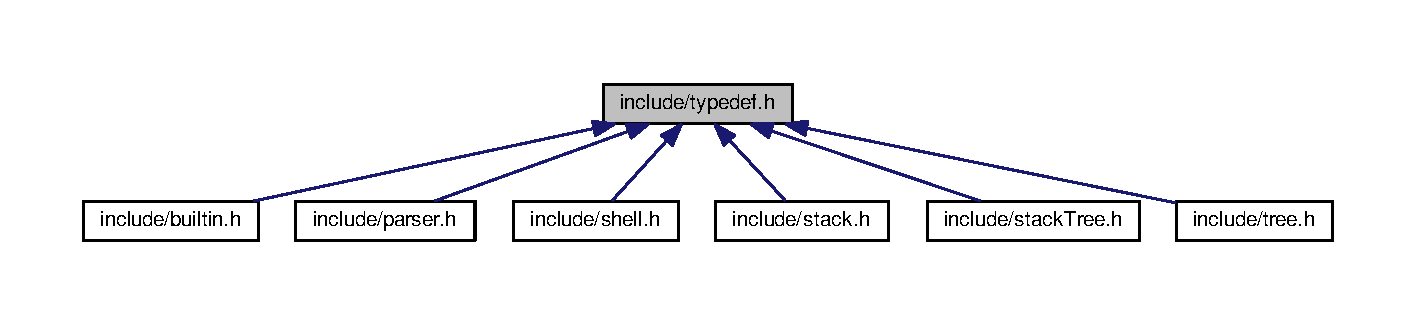
\includegraphics[width=350pt]{typedef_8h__dep__incl}
\end{center}
\end{figure}
\subsection*{Classes}
\begin{DoxyCompactItemize}
\item 
struct \hyperlink{structnode}{node}
\item 
struct \hyperlink{structstackNode}{stack\+Node}
\begin{DoxyCompactList}\small\item\em Structure noeud de pile contenant la donnee et le noeud suivant. \end{DoxyCompactList}\item 
struct \hyperlink{structstackTree}{stack\+Tree}
\begin{DoxyCompactList}\small\item\em Structure pile d\textquotesingle{}arbre contenant un arbre et l\textquotesingle{}arbre suivant. \end{DoxyCompactList}\end{DoxyCompactItemize}
\subsection*{Macros}
\begin{DoxyCompactItemize}
\item 
\#define \hyperlink{typedef_8h_af1abcb51a4aa27a5a5a7958c03448134}{M\+A\+X\+\_\+\+C\+O\+M\+M\+A\+N\+D\+\_\+\+L\+E\+N\+G\+TH}~150
\item 
\#define {\bfseries M\+A\+X\+\_\+\+N\+U\+M\+B\+E\+R\+\_\+\+O\+F\+\_\+\+P\+A\+R\+A\+MS}~30\hypertarget{typedef_8h_a093500fedd419f3091cfb430da6165a0}{}\label{typedef_8h_a093500fedd419f3091cfb430da6165a0}

\item 
\#define {\bfseries M\+A\+X\+\_\+\+N\+U\+M\+B\+E\+R\+\_\+\+O\+F\+\_\+\+C\+MD}~30\hypertarget{typedef_8h_a93d1e42f20aca136db885b3ac86c2a18}{}\label{typedef_8h_a93d1e42f20aca136db885b3ac86c2a18}

\item 
\#define {\bfseries S\+T\+D\+IN}~0\hypertarget{typedef_8h_ac00bfb46347d26fdc58568fe1ab5fa5b}{}\label{typedef_8h_ac00bfb46347d26fdc58568fe1ab5fa5b}

\item 
\#define {\bfseries S\+T\+D\+O\+UT}~1\hypertarget{typedef_8h_a8875037d0772a4fc34516f1e03d7e238}{}\label{typedef_8h_a8875037d0772a4fc34516f1e03d7e238}

\item 
\#define {\bfseries S\+T\+D\+E\+RR}~2\hypertarget{typedef_8h_a3a540e3eef339eec06aff31c4ba1eb25}{}\label{typedef_8h_a3a540e3eef339eec06aff31c4ba1eb25}

\item 
\#define {\bfseries K\+N\+RM}~\char`\"{}\textbackslash{}x1B\mbox{[}0m\char`\"{}\hypertarget{typedef_8h_a137aa83ec74421d226a90c92ec032ac9}{}\label{typedef_8h_a137aa83ec74421d226a90c92ec032ac9}

\item 
\#define {\bfseries K\+R\+ED}~\char`\"{}\textbackslash{}x1B\mbox{[}31m\char`\"{}\hypertarget{typedef_8h_a66290957baed5df3930ada4cb8caccf1}{}\label{typedef_8h_a66290957baed5df3930ada4cb8caccf1}

\item 
\#define {\bfseries K\+G\+RN}~\char`\"{}\textbackslash{}x1B\mbox{[}32m\char`\"{}\hypertarget{typedef_8h_ac081c83b067273757f7a2e54a5957d41}{}\label{typedef_8h_ac081c83b067273757f7a2e54a5957d41}

\item 
\#define {\bfseries K\+Y\+EL}~\char`\"{}\textbackslash{}x1B\mbox{[}33m\char`\"{}\hypertarget{typedef_8h_a897b10d246533c95ba86cb79f92e465a}{}\label{typedef_8h_a897b10d246533c95ba86cb79f92e465a}

\item 
\#define {\bfseries K\+B\+LU}~\char`\"{}\textbackslash{}x1B\mbox{[}34m\char`\"{}\hypertarget{typedef_8h_a3f838f2fc3a9a3b434be606fc908964b}{}\label{typedef_8h_a3f838f2fc3a9a3b434be606fc908964b}

\item 
\#define {\bfseries K\+M\+AG}~\char`\"{}\textbackslash{}x1B\mbox{[}35m\char`\"{}\hypertarget{typedef_8h_a6825f05d3b9d619d91d79d0ef18bb8b2}{}\label{typedef_8h_a6825f05d3b9d619d91d79d0ef18bb8b2}

\item 
\#define {\bfseries K\+C\+YN}~\char`\"{}\textbackslash{}x1B\mbox{[}36m\char`\"{}\hypertarget{typedef_8h_a32036c94dbb166a3f874b7efc169841f}{}\label{typedef_8h_a32036c94dbb166a3f874b7efc169841f}

\item 
\#define {\bfseries K\+W\+HT}~\char`\"{}\textbackslash{}x1B\mbox{[}37m\char`\"{}\hypertarget{typedef_8h_af0036c8022c9980079ab17e5c87fd478}{}\label{typedef_8h_af0036c8022c9980079ab17e5c87fd478}

\item 
\#define {\bfseries B\+O\+LD}~\char`\"{}\textbackslash{}x1B\mbox{[}1m\char`\"{}\hypertarget{typedef_8h_a26cdbb1a00213c810caccf21cd33a631}{}\label{typedef_8h_a26cdbb1a00213c810caccf21cd33a631}

\end{DoxyCompactItemize}
\subsection*{Typedefs}
\begin{DoxyCompactItemize}
\item 
typedef struct \hyperlink{structnode}{node} $\ast$ {\bfseries Tree}\hypertarget{typedef_8h_a65cc6ee99f44c5fe2972d8ee7d895f68}{}\label{typedef_8h_a65cc6ee99f44c5fe2972d8ee7d895f68}

\item 
typedef struct \hyperlink{structstackNode}{stack\+Node} $\ast$ {\bfseries Stack}\hypertarget{typedef_8h_ad0aa4d116a878fdd7dcc9c82b4cb5446}{}\label{typedef_8h_ad0aa4d116a878fdd7dcc9c82b4cb5446}

\item 
typedef struct \hyperlink{structstackTree}{stack\+Tree} $\ast$ {\bfseries Stack\+Tree}\hypertarget{typedef_8h_a096a0a245198f21b66ce18ce1511fa23}{}\label{typedef_8h_a096a0a245198f21b66ce18ce1511fa23}

\end{DoxyCompactItemize}
\subsection*{Enumerations}
\begin{DoxyCompactItemize}
\item 
enum \hyperlink{typedef_8h_af6a258d8f3ee5206d682d799316314b1}{bool} \{ {\bfseries true}, 
{\bfseries false}
 \}\hypertarget{typedef_8h_af6a258d8f3ee5206d682d799316314b1}{}\label{typedef_8h_af6a258d8f3ee5206d682d799316314b1}
\begin{DoxyCompactList}\small\item\em Booléen. \end{DoxyCompactList}
\end{DoxyCompactItemize}


\subsection{Detailed Description}
Définition des types. 

\begin{DoxyAuthor}{Author}
Loïc.\+B et Jean.\+S
\end{DoxyAuthor}
Définitions des types 

\subsection{Macro Definition Documentation}
\index{typedef.\+h@{typedef.\+h}!M\+A\+X\+\_\+\+C\+O\+M\+M\+A\+N\+D\+\_\+\+L\+E\+N\+G\+TH@{M\+A\+X\+\_\+\+C\+O\+M\+M\+A\+N\+D\+\_\+\+L\+E\+N\+G\+TH}}
\index{M\+A\+X\+\_\+\+C\+O\+M\+M\+A\+N\+D\+\_\+\+L\+E\+N\+G\+TH@{M\+A\+X\+\_\+\+C\+O\+M\+M\+A\+N\+D\+\_\+\+L\+E\+N\+G\+TH}!typedef.\+h@{typedef.\+h}}
\subsubsection[{\texorpdfstring{M\+A\+X\+\_\+\+C\+O\+M\+M\+A\+N\+D\+\_\+\+L\+E\+N\+G\+TH}{MAX_COMMAND_LENGTH}}]{\setlength{\rightskip}{0pt plus 5cm}\#define M\+A\+X\+\_\+\+C\+O\+M\+M\+A\+N\+D\+\_\+\+L\+E\+N\+G\+TH~150}\hypertarget{typedef_8h_af1abcb51a4aa27a5a5a7958c03448134}{}\label{typedef_8h_af1abcb51a4aa27a5a5a7958c03448134}
Variable globale, gere la taille des differents tableaux du shell 
%--- End generated contents ---

% Index
\backmatter
\newpage
\phantomsection
\clearemptydoublepage
\addcontentsline{toc}{chapter}{Index}
\printindex

\end{document}
